
\documentclass[border=5pt]{standalone}
\usepackage[utf8]{inputenc}
\usepackage[T1]{fontenc}
\usepackage{amsmath,amssymb}
\usepackage{tikz}
\usetikzlibrary{arrows.meta,shapes.misc,calc}
\renewcommand{\familydefault}{\sfdefault}
\tikzset{
  ptcross/.style={cross out,draw,thick,minimum size=1.6mm,inner sep=0pt},
  vec/.style={->,thick,>={Stealth[length=2.6mm]}},
  vecu/.style={vec,color=blue!70!black},
  vecv/.style={vec,color=red!75!black},
  vecw/.style={vec,color=green!45!black},
  grid/.style={gray!35,thin},
}
\newcommand{\Vj}[1]{\overrightarrow{\text{#1}}}
\newcommand{\pt}[4]{\node[ptcross] at (#1,#2) {}; \node[anchor=#4,inner sep=2pt] at (#1,#2) {$#3$};}
\begin{document}
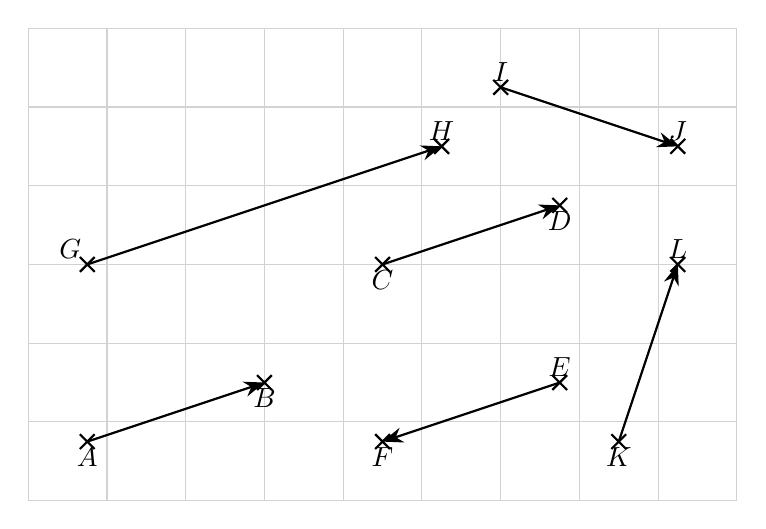
\begin{tikzpicture}[x=0.75cm,y=0.75cm]
\draw[grid] (0,0) grid (12,8);
\draw[vec] (1,1) -- (4,2);
\pt{1}{1}{A}{north}
\pt{4}{2}{B}{north}
\draw[vec] (6,4) -- (9,5);
\pt{6}{4}{C}{north}
\pt{9}{5}{D}{north}
\draw[vec] (9,2) -- (6,1);
\pt{9}{2}{E}{south}
\pt{6}{1}{F}{north}
\draw[vec] (1,4) -- (7,6);
\pt{1}{4}{G}{south east}
\pt{7}{6}{H}{south}
\draw[vec] (8,7) -- (11,6);
\pt{8}{7}{I}{south}
\pt{11}{6}{J}{south}
\draw[vec] (10,1) -- (11,4);
\pt{10}{1}{K}{north}
\pt{11}{4}{L}{south}

\end{tikzpicture}
\end{document}
